%%%%%%%%%%%%%%%%%%%%%%%%%%%%%%%%%%%%%%%%%%%%%%%%%%%%%%%%%%%%%%%%%%%%%%%%%%%%%%%%%
% Template: Exam
%
% Por: Abrantes Araújo Silva Filho
%      abrantesasf@gmail.com
%
% Citação: Se você gostou deste template, por favor ajude a divulgá-lo mantendo
%          o link para meu repositório GitHub em:
%          https://github.com/abrantesasf/LaTeX
%%%%%%%%%%%%%%%%%%%%%%%%%%%%%%%%%%%%%%%%%%%%%%%%%%%%%%%%%%%%%%%%%%%%%%%%%%%%%%%%%




%%%%%%%%%%%%%%%%%%%%%%%%%%%%%%%%%%%%%%%%%%%%%%%%%%%%%%%%%%%%%%%%%%%%%%%%%%%%%%%%%
%%% Configura o tipo de documento, papel, tamanho da fonte e informações básicas
%%% para as proriedades do PDF/DVIPS e outras propriedades do documento
\RequirePackage{ifpdf}
\ifpdf
  % Classe, língua e tamanho da fonte padrão. Outras opções a considerar:
  %   draft
  %   onecolumn (padrão) ou twocolumn (OU usar o package multicol)
  %   fleqn com ou sem leqno (alinhamento à esquerda das fórmulas e dos números)
  %   oneside (padrão para article ou report) ou twoside (padrão para book)
  %   answers = imprime respostas para o gabarito
  \documentclass[pdftex, brazil, 12pt, oneside, addpoints]{exam}
\else
  % Classe, língua e tamanho da fonte padrão. Outras opções a considerar:
  %   draft
  %   onecolumn (padrão) ou twocolumn (OU usar o package multicol)
  %   fleqn com ou sem leqno (alinhamento à esquerda das fórmulas e dos números)
  %   oneside (padrão para article ou report) ou twoside (padrão para book)
  %   answers = imprime respostas para o gabarito
  \documentclass[brazil, 12pt, oneside, addpoints]{exam}
\fi


%%%%%%%%%%%%%%%%%%%%%%%%%%%%%%%%%%%%%%%%%%%%%%%%%%%%%%%%%%%%%%%%%%%%%%%%%%%%%%%%%
%%% Carrega pacotes iniciais necessários para estrutura de controle e para a
%%% criação e o parse de novos comandos
\usepackage{ifthen}
\usepackage{xparse}


%%%%%%%%%%%%%%%%%%%%%%%%%%%%%%%%%%%%%%%%%%%%%%%%%%%%%%%%%%%%%%%%%%%%%%%%%%%%%%%%%
%%% Configuração do tamanho da página, margens, espaçamento entrelinhas e, se
%%% necessário, ativa a indentação dos primeiros parágrafos.
\ifpdf
  \usepackage[pdftex]{geometry}
\else
  \usepackage[dvips]{geometry}
\fi
\geometry{a4paper, left=2.0cm, right=2.0cm, top=2.0cm, bottom=2.0cm}

\usepackage{setspace}
  \singlespacing
  %\onehalfspacing
  %\doublespacing


%%%%%%%%%%%%%%%%%%%%%%%%%%%%%%%%%%%%%%%%%%%%%%%%%%%%%%%%%%%%%%%%%%%%%%%%%%%%%%%%%
%%% Configurações de encoding, lingua e fontes:
\usepackage[T1]{fontenc}
\usepackage[utf8]{inputenc}
\usepackage{babel}

% Altera a fonte padrão do documento (nem todas funcionam em modo math):
%   phv = Helvetica
%   ptm = Times
%   ppl = Palatino
%   pbk = bookman
%   pag = AdobeAvantGarde
%   pnc = Adobe NewCenturySchoolBook
\renewcommand{\familydefault}{ppl}


%%%%%%%%%%%%%%%%%%%%%%%%%%%%%%%%%%%%%%%%%%%%%%%%%%%%%%%%%%%%%%%%%%%%%%%%%%%%%%%%%
%%% Configurações de cabeçalho e rodapé (não pode usar fancyhdr pois ocorre conflito):
\pagestyle{headandfoot}
\runningheadrule
\firstpageheader{}{}{}
\runningheader{Exercício 0: revisão de matemática}{}{Agosto/2019}
\firstpagefooter{}{}{Página \thepage\ de \numpages}
\runningfooter{}{}{Página \thepage\ de \numpages}
\runningfootrule


%%%%%%%%%%%%%%%%%%%%%%%%%%%%%%%%%%%%%%%%%%%%%%%%%%%%%%%%%%%%%%%%%%%%%%%%%%%%%%%%%
%%% Carrega bibliotecas de símbolos (matemáticos, físicos, etc.), fontes
%%% adicionais, e configura algumas opções
\usepackage{amsmath}
\usepackage{amssymb}
\usepackage{amsfonts}
\usepackage{siunitx}
  \sisetup{group-separator = {.}}
  \sisetup{group-digits = {false}}
  \sisetup{output-decimal-marker = {,}}
\usepackage{bm}
\usepackage{cancel}
% Altera separador decimal via comando, se necessário (prefira o siunitx):
%\mathchardef\period=\mathcode`.
%\DeclareMathSymbol{.}{\mathord}{letters}{"3B}


%%%%%%%%%%%%%%%%%%%%%%%%%%%%%%%%%%%%%%%%%%%%%%%%%%%%%%%%%%%%%%%%%%%%%%%%%%%%%%%%%
%%% Carrega pacotes para referências cruzadas, citações dentro do documento,
%%% links para internet e outros.Configura algumas opções.
%%% Não altere a ordem de carregamento dos packages.
\usepackage{varioref}
\ifpdf
  \usepackage[pdftex]{hyperref}
    \hypersetup{
      % Informações variáveis em cada documento (MUDE AQUI!):
      pdftitle={Exercício 0: revisão de matemática},
      pdfauthor={Abrantes Araújo Silva Filho},
      pdfsubject={Revisão de matemática},
      pdfkeywords={matemática, revisão},
      pdfinfo={
        CreationDate={}, % Ex.: D:AAAAMMDDHH24MISS
        ModDate={}       % Ex.: D:AAAAMMDDHH24MISS
      },
      % Coisas que você não deve alterar se não souber o que está fazendo:
      unicode=true,
      pdflang={pt-BR},
      bookmarksopen=true,
      bookmarksnumbered=true,
      bookmarksopenlevel=5,
      pdfdisplaydoctitle=true,
      pdfpagemode=UseOutlines,
      pdfstartview=FitH,
      pdfcreator={LaTeX with hyperref package},
      pdfproducer={pdfTeX},
      pdfnewwindow=true,
      colorlinks=true,
      citecolor=green,
      linkcolor=red,
      filecolor=cyan,
      urlcolor=blue
    }
\else
  \usepackage{hyperref}
\fi
\usepackage{cleveref}
\usepackage{url}
  

%%%%%%%%%%%%%%%%%%%%%%%%%%%%%%%%%%%%%%%%%%%%%%%%%%%%%%%%%%%%%%%%%%%%%%%%%%%%%%%%%
%%% Carrega packages relacionados à computação
\usepackage{algorithm2e}
\usepackage{algorithmicx}
\usepackage{algpseudocode}
\usepackage{listings}
  \lstset{literate=
    {á}{{\'a}}1 {é}{{\'e}}1 {í}{{\'i}}1 {ó}{{\'o}}1 {ú}{{\'u}}1
    {Á}{{\'A}}1 {É}{{\'E}}1 {Í}{{\'I}}1 {Ó}{{\'O}}1 {Ú}{{\'U}}1
    {à}{{\`a}}1 {è}{{\`e}}1 {ì}{{\`i}}1 {ò}{{\`o}}1 {ù}{{\`u}}1
    {À}{{\`A}}1 {È}{{\'E}}1 {Ì}{{\`I}}1 {Ò}{{\`O}}1 {Ù}{{\`U}}1
    {ä}{{\"a}}1 {ë}{{\"e}}1 {ï}{{\"i}}1 {ö}{{\"o}}1 {ü}{{\"u}}1
    {Ä}{{\"A}}1 {Ë}{{\"E}}1 {Ï}{{\"I}}1 {Ö}{{\"O}}1 {Ü}{{\"U}}1
    {â}{{\^a}}1 {ê}{{\^e}}1 {î}{{\^i}}1 {ô}{{\^o}}1 {û}{{\^u}}1
    {Â}{{\^A}}1 {Ê}{{\^E}}1 {Î}{{\^I}}1 {Ô}{{\^O}}1 {Û}{{\^U}}1
    {œ}{{\oe}}1 {Œ}{{\OE}}1 {æ}{{\ae}}1 {Æ}{{\AE}}1 {ß}{{\ss}}1
    {ű}{{\H{u}}}1 {Ű}{{\H{U}}}1 {ő}{{\H{o}}}1 {Ő}{{\H{O}}}1
    {ç}{{\c c}}1 {Ç}{{\c C}}1 {ø}{{\o}}1 {å}{{\r a}}1 {Å}{{\r A}}1
    {€}{{\euro}}1 {£}{{\pounds}}1 {«}{{\guillemotleft}}1
    {»}{{\guillemotright}}1 {ñ}{{\~n}}1 {Ñ}{{\~N}}1 {¿}{{?`}}1
  }
  

%%%%%%%%%%%%%%%%%%%%%%%%%%%%%%%%%%%%%%%%%%%%%%%%%%%%%%%%%%%%%%%%%%%%%%%%%%%%%%%%%
%%% Ativa suporte extendido a cores
\usepackage[svgnames]{xcolor} % Opções de cores: usenames (16), dvipsnames (64),
                              % svgnames (150) e x11names (300).


%%%%%%%%%%%%%%%%%%%%%%%%%%%%%%%%%%%%%%%%%%%%%%%%%%%%%%%%%%%%%%%%%%%%%%%%%%%%%%%%%
%%% Suporte à importação de gráficos externos
\ifpdf
  \usepackage[pdftex]{graphicx}
\else
  \usepackage[dvips]{graphicx}
\fi


%%%%%%%%%%%%%%%%%%%%%%%%%%%%%%%%%%%%%%%%%%%%%%%%%%%%%%%%%%%%%%%%%%%%%%%%%%%%%%%%%
%%% Suporte à criação de gráficos proceduralmente na LaTeX:
\usepackage{tikz}
  \usetikzlibrary{arrows,automata,backgrounds,matrix,patterns,positioning,shapes,shadows}


%%%%%%%%%%%%%%%%%%%%%%%%%%%%%%%%%%%%%%%%%%%%%%%%%%%%%%%%%%%%%%%%%%%%%%%%%%%%%%%%%
%%% Packages para tabelas
\usepackage{array}
\usepackage{longtable}
\usepackage{tabularx}
\usepackage{tabu}
\usepackage{lscape}
\usepackage{colortbl}  
\usepackage{booktabs}
\newcolumntype{M}[1]{>{\centering\arraybackslash}m{#1}}
%\newcolumntype{ML}[1]{>{$}l<{$}}
%\newcolumntype{MR}[1]{>{R}r<{R}}
\newcolumntype{L}[1]{>{\arraybackslash}m{#1}}
\newcolumntype{N}{@{}m{0pt}@{}}


%%%%%%%%%%%%%%%%%%%%%%%%%%%%%%%%%%%%%%%%%%%%%%%%%%%%%%%%%%%%%%%%%%%%%%%%%%%%%%%%%
%%% Packages ambientes de listas
\usepackage{enumitem}
\usepackage[ampersand]{easylist}


%%%%%%%%%%%%%%%%%%%%%%%%%%%%%%%%%%%%%%%%%%%%%%%%%%%%%%%%%%%%%%%%%%%%%%%%%%%%%%%%%
%%% Packages para suporte a ambientes floats, captions, etc.:
\usepackage{float}
\usepackage{wrapfig}
\usepackage{placeins}
\usepackage{caption}
\usepackage{sidecap}
\usepackage{subcaption}


%%%%%%%%%%%%%%%%%%%%%%%%%%%%%%%%%%%%%%%%%%%%%%%%%%%%%%%%%%%%%%%%%%%%%%%%%%%%%%%%%
%%% Meus comandos específicos:
% Commando para ``italizar´´ palavras em inglês (e outras línguas!):
\newcommand{\ingles}[1]{\textit{#1}}

% Commando para colocar o espaço correto entre um número e sua unidade:
\newcommand{\unidade}[2]{\ensuremath{#1\,\mathrm{#2}}}
\newcommand{\unidado}[2]{{#1}\,{#2}}

% Produz ordinal masculino ou feminino dependendo do segundo argumento:
\newcommand{\ordinal}[2]{%
#1%
\ifthenelse{\equal{a}{#2}}%
{\textordfeminine}%
{\textordmasculine}}


%%%%%%%%%%%%%%%%%%%%%%%%%%%%%%%%%%%%%%%%%%%%%%%%%%%%%%%%%%%%%%%%%%%%%%%%%%%%%%%%%
%%% Hifenização específica quando o LaTeX/Babel não conseguirem hifenizar:
\babelhyphenation{Git-Hub}


%%%%%%%%%%%%%%%%%%%%%%%%%%%%%%%%%%%%%%%%%%%%%%%%%%%%%%%%%%%%%%%%%%%%%%%%%%%%%%%%%
%%% Comandos específicos para a classe EXAM deste documento:
\newcommand{\umalinha}{\fillwithlines{0.25in}}
\newcommand{\duaslinhas}{\fillwithlines{0.50in}}
\newcommand{\treslinhas}{\fillwithlines{0.75in}}
\newcommand{\quatrolinhas}{\fillwithlines{1.00in}}
\newcommand{\cincolinhas}{\fillwithlines{1.25in}}
\newcommand{\seislinhas}{\fillwithlines{1.50in}}
\newcommand{\setelinhas}{\fillwithlines{1.75in}}
\newcommand{\oitolinhas}{\fillwithlines{2.00in}}
\newcommand{\novelinhas}{\fillwithlines{2.25in}}
\newcommand{\dezlinhas}{\fillwithlines{2.50in}}

% Verdadeiro ou Falvo para a classe EXAM
\newcommand{\vf}[1][{}]{%
  \fillin[#1][0.25in]%
}

% Título das respostas:
%\renewcommand{\solutiontitle}{\noindent\textbf{Resposta:}\par\noindent}
\renewcommand{\solutiontitle}{\noindent}
%\shadedsolutions
%\SolutionEmphasis{\itshape}




%%%%%%%%%%%%%%%%%%%%%%%%%%%%%%%%%%%%%%%%%%%%%%%%%%%%%%%%%%%%%%%%%%%%%%%%%%%%%%%%%
%%%%%%%%%%%%%%%%%%%%%%%%%%%%%%%%%%%%%%%%%%%%%%%%%%%%%%%%%%%%%%%%%%%%%%%%%%%%%%%%%
%%%%%%%%%%%%%%%%%%%%%%%%%%%%%%%%%%%%%%%%%%%%%%%%%%%%%%%%%%%%%%%%%%%%%%%%%%%%%%%%%
%%%%%%%%%%%%%%%%%%%%%%%%%%%%%%%%%%%%%%%%%%%%%%%%%%%%%%%%%%%%%%%%%%%%%%%%%%%%%%%%%
%%%%%%%%%%%%%%%%%%%%%%%%%%%%%% COMEÇA O DOCUMENTO %%%%%%%%%%%%%%%%%%%%%%%%%%%%%%%
%%%%%%%%%%%%%%%%%%%%%%%%%%%%%%%%%%%%%%%%%%%%%%%%%%%%%%%%%%%%%%%%%%%%%%%%%%%%%%%%%
%%%%%%%%%%%%%%%%%%%%%%%%%%%%%%%%%%%%%%%%%%%%%%%%%%%%%%%%%%%%%%%%%%%%%%%%%%%%%%%%%
%%%%%%%%%%%%%%%%%%%%%%%%%%%%%%%%%%%%%%%%%%%%%%%%%%%%%%%%%%%%%%%%%%%%%%%%%%%%%%%%%
%%%%%%%%%%%%%%%%%%%%%%%%%%%%%%%%%%%%%%%%%%%%%%%%%%%%%%%%%%%%%%%%%%%%%%%%%%%%%%%%%
\begin{document}


%%%%%%%%%%%%%%%%%%%%%%%%%%%%%%%%%%%%%%%%%%%%%%%%%%%%%%%%%%%%%%%%%%%%%%%%%%%%%%%%%
%%%%%%%%%%%%%%%%%%%%%%%%%%%%%%%%%%%%%%%%%%%%%%%%%%%%%%%%%%%%%%%%%%%%%%%%%%%%%%%%%
%%%%%%%%%%%%%%%%%%%%%%%%%%%%%%%%%%%%%%%%%%%%%%%%%%%%%%%%%%%%%%%%%%%%%%%%%%%%%%%%%
\begin{coverpages}

\begin{center}
\textbf{\textit{\Large%
Álgebra Linear\\
--- monitoria ---}}
\end{center}

\vspace{1cm}

\begin{figure}[H]
\begin{center}
\fbox{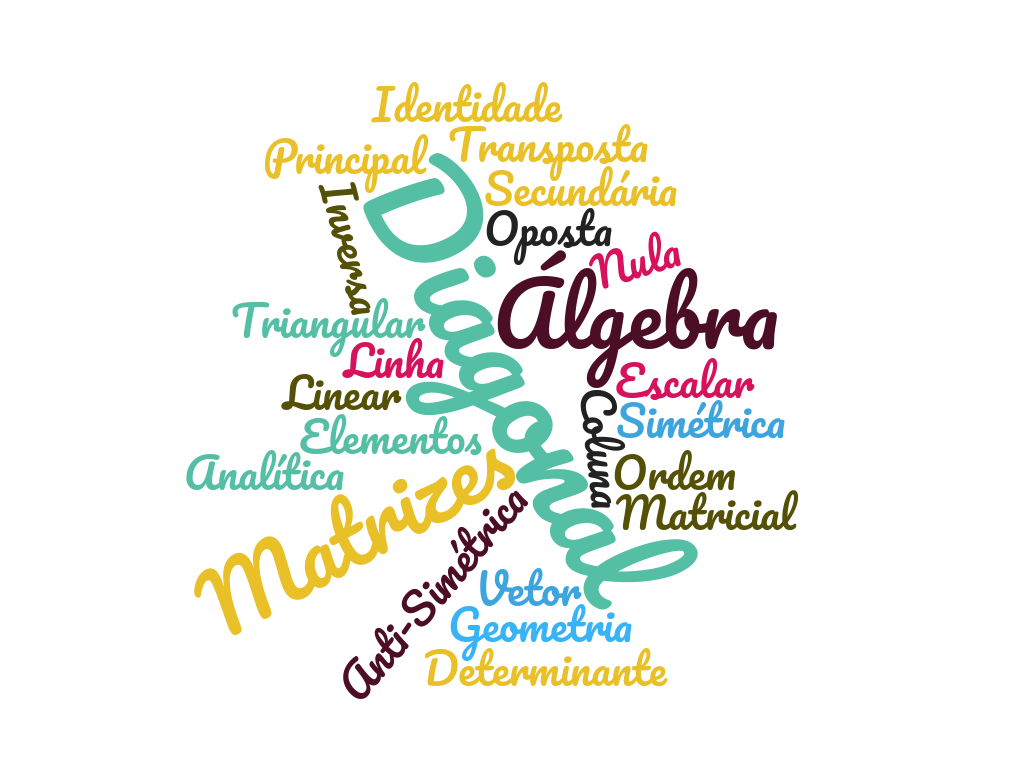
\includegraphics[scale=0.4]{linear_algebra.png}}
\end{center}
\end{figure}

\vspace{1cm}

\begin{center}
\textit{\textbf{\Large%
--- Exercício 0: revisão de matemática ---\\
\ \\
Agosto/2019}}
\end{center}

%\vspace{1cm}
%\begin{flushright}
%\textbf{Monitor(es):}\\
%\textit{Monitor 1\\
%Monitor 2}
%\end{flushright}

%\begin{center}
%  \fbox{\fbox{\parbox{5.5in}{\centering
%        Answer the questions in the spaces provided on the
%        question sheets. If you run out of room for an answer,
%        continue on the back of the page.}}}
%\end{center}

\end{coverpages}

\newpage

Os exercícios a seguir têm o objetivo de garantir que você esteja preparado para
a disciplina de Álgebra Linear (e outras como: cálculo, física, matemática
discreta, etc\ldots). Esses exercícios não são obrigatórios mas são importantes
para que você mesmo avalie sua capacidade matemática e descubra onde precisa
revisar e melhorar.

Todos os exercícios abaixo foram retirados do livro do George F.\ Simmons:
\ingles{Precalculus Mathematics in a Nutshell: Geometry, Algebra, Trigonometry},
republicado pela Wipf \& Stock Publishers, em 2003\footnote{A edição original é de
1987 e continua sendo um dos melhores livros para revisão de matemática que eu
conheço. Ainda está disponível para compra na Amazon: \url{https://www.amazon.com/Precalculus-Mathematics-Nutshell-Geometry-Trigonometry/dp/1592441300/}}:

\begin{figure}[H]
  \begin{center}
    \caption{\ingles{Precalculus}, do Simmons}
    \label{fig:simmons}
    \fbox{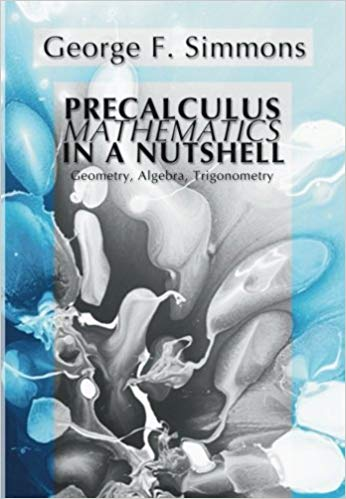
\includegraphics[scale=0.3]{simmons.jpg}}
    %\footnotesize{Fonte:~}
  \end{center}
\end{figure}

\begin{questions}
\setlength\linefillthickness{0.2pt}
%%%%%%%%%%%%%%%%%%%%%%%%%%%%%%%%%%%%%%%%%%%%%%%%%%%%%%%%%%%%%%%%%%%%%%%%%%%%%%%%%
%%%%%%%%%%%%%%%%%%%%%%%%%%%%%%%%%%%%%%%%%%%%%%%%%%%%%%%%%%%%%%%%%%%%%%%%%%%%%%%%%
%%%%%%%%%%%%%%%%%%%%%%%%%%%%%%%%%%%%%%%%%%%%%%%%%%%%%%%%%%%%%%%%%%%%%%%%%%%%%%%%%
\fullwidth{\section{Be-a-bá matemático}}
%\ifprintanswers
%\newpage
%\else
%\newpage
%\fi

\question
Identifique a qual conjunto numérico os seguintes números pertencem:
\begin{parts}
  \part $\sqrt{9}$
  \part $-\cfrac{2}{3}$
  \part $\cfrac{51}{3}$
  \part $-10$
  \part $-\cfrac{\pi}{3}$
  \part $\cfrac{\sqrt{5}}{2}$
  \part $-\sqrt{4}$
  \part $\cfrac{5}{1234}$
\end{parts}

\question
Simplifique:
\begin{parts}
  \part $(3a - b) - [2a - (a + b)]$
  \part $[(a + 3b) - a] - [a - (a - 3b)]$
  \part $a - \{2a - [b - (3a - 2b)]\}$
\end{parts}

\question
Simplifique removendo fatores comuns:
\begin{parts}
  \part $12x - 18y + 30$
  \part $8x^2 - 12x^3y - 28x^4z$
  \part $9abc + 3a^2b^2c^2$
\end{parts}

\question
Resolva e simplifique:
\begin{parts}
  \part $\cfrac{a}{b} - \cfrac{b}{a}$
  \part $\cfrac{3}{x-2} + \cfrac{1}{2-x}$
  \part $\cfrac{1}{1 + \cfrac{1}{x-1}}$
  \part $\cfrac{x}{xy^2} + \cfrac{y}{x^2y}$
  \part $\cfrac{4a}{b} + \cfrac{b}{4a}$
\end{parts}


%%%%%%%%%%%%%%%%%%%%%%%%%%%%%%%%%%%%%%%%%%%%%%%%%%%%%%%%%%%%%%%%%%%%%%%%%%%%%%%%%
%%%%%%%%%%%%%%%%%%%%%%%%%%%%%%%%%%%%%%%%%%%%%%%%%%%%%%%%%%%%%%%%%%%%%%%%%%%%%%%%%
%%%%%%%%%%%%%%%%%%%%%%%%%%%%%%%%%%%%%%%%%%%%%%%%%%%%%%%%%%%%%%%%%%%%%%%%%%%%%%%%%
\fullwidth{\section{Potenciação}}
%\ifprintanswers
%\newpage
%\else
%\newpage
%\fi

\question
Simplifique removendo expoentes negativos e zero:
\begin{parts}
  \part $5a^{-3}$
  \part $(5a)^{-3}$
  \part $21 \times 719^3 \times 7^{-1} \times 3 \times 719^{-3}$
  \part $\left[\cfrac{2a^{-3} + 3a^{-2}}{3a^{-4} + 4a^{-3}}\right]^0$
\end{parts}

\question
Simplifique:
\begin{parts}
  \part $(a^{n-4}b^4)(ab^{n-1})^4$
  \part $(4a^3b^{-4})(3a^{-1}b^5)$
  \part $\cfrac{x^{14}y^5}{x^4y^{-5}}$
  \part $a^2b^2(a^{-2} + b^{-2})$
  \part $(x + y)(x^{-1} + y^{-1})$
  \part $\left(\cfrac{a^2b}{c}\right)^4\left(\cfrac{a}{b^2c^3}\right)^2\left(\cfrac{c^2}{a^5}\right)^5$
\end{parts}


%%%%%%%%%%%%%%%%%%%%%%%%%%%%%%%%%%%%%%%%%%%%%%%%%%%%%%%%%%%%%%%%%%%%%%%%%%%%%%%%%
%%%%%%%%%%%%%%%%%%%%%%%%%%%%%%%%%%%%%%%%%%%%%%%%%%%%%%%%%%%%%%%%%%%%%%%%%%%%%%%%%
%%%%%%%%%%%%%%%%%%%%%%%%%%%%%%%%%%%%%%%%%%%%%%%%%%%%%%%%%%%%%%%%%%%%%%%%%%%%%%%%%
\fullwidth{\section{Radiciação}}
%\ifprintanswers
%\newpage
%\else
%\newpage
%\fi

\question
Simplifique sem usar a calculadora:
\begin{parts}
  \part $\sqrt{49}$
  \part $\sqrt{144}$
  \part $\sqrt{9 + 16}$
  \part $\sqrt{36 + 64}$
  \part $\sqrt[3]{27}$
  \part $\sqrt[4]{81}$
  \part $\sqrt[6]{64}$
  \part $\sqrt{0.64}$
  \part $\sqrt{0.09}$
  \part $\sqrt{\cfrac{16}{121}}$
  \part $\sqrt{\cfrac{225}{400}}$
  \part $\sqrt[3]{-\cfrac{1}{27}}$
  \part $\sqrt[3]{\cfrac{64}{125}}$
  \part $\sqrt[3]{-1000}$
  \part $\sqrt{125}$
  \part $\sqrt{625}$
  \part $\sqrt[4]{625}$
  \part $\sqrt{18}$
  \part $\sqrt{12}$
  \part $\sqrt{2} + \sqrt{8}$
  \part $\sqrt{3} + \sqrt[4]{9}$
  \part $\sqrt[3]{54} + \sqrt[3]{250}$
  \part $\sqrt[10]{32a^5}$
  \part $\sqrt{a^2b^4}$
  \part $\sqrt[4]{a^5}$
  \part $\sqrt{1-\left(\cfrac{\sqrt{3}}{2}\right)^2}$
\end{parts}

\question
Simplifique racionalizando o denominador:
\begin{parts}
  \part $\cfrac{30}{\sqrt{6}}$
  \part $\cfrac{\sqrt{6} + 2}{\sqrt{6} - 2}$
  \part $\cfrac{2}{\sqrt{7} + \sqrt{5}}$
  \part $\cfrac{3}{\sqrt[3]{2^7}}$
\end{parts}


%%%%%%%%%%%%%%%%%%%%%%%%%%%%%%%%%%%%%%%%%%%%%%%%%%%%%%%%%%%%%%%%%%%%%%%%%%%%%%%%%
%%%%%%%%%%%%%%%%%%%%%%%%%%%%%%%%%%%%%%%%%%%%%%%%%%%%%%%%%%%%%%%%%%%%%%%%%%%%%%%%%
%%%%%%%%%%%%%%%%%%%%%%%%%%%%%%%%%%%%%%%%%%%%%%%%%%%%%%%%%%%%%%%%%%%%%%%%%%%%%%%%%
\fullwidth{\section{Potências e raízes}}
%\ifprintanswers
%\newpage
%\else
%\newpage
%\fi

\question
Calcule:
\begin{parts}
  \part $36^{1/2}$
  \part $8^{1/3}$
  \part $32^{4/5}$
  \part $36^{3/2}$
  \part $216^{2/3}$
  \part $16^{-1/2}$
  \part $9^{-3/2}$
  \part $8^{-2/3}$
  \part $100^{3/2}$
  \part $3^{1/2} \times 3^{5/2}$
  \part $\cfrac{10^{2/3} \times 10^{1/3} \times 10^{3}}{10^{5/2} \times 10^{1/2}}$
\end{parts}

\question
Simplifique o máximo possível:
\begin{parts}
  \part $(25a^6b^{-2})^{1/2}$
  \part $(2a^{1/2}b^{1/4})^4$
  \part $\sqrt[5]{a^2b} \times \sqrt[5]{a^3b^4}$
  \part $\left(\cfrac{a^4}{36}\right)^{1/2}$
  \part $(25a^{2/3})^{1/2}$
  \part $(a^{1/2} + b^{1/2})(a^{1/2} - b^{1/2})$
  \part $\left\{a^{2/3}\left[\left(\cfrac{a^{2/3}}{a^{1/4}}\right)^6\right]^{1/3}\right\}^2$
  \part $\left(\cfrac{27b^2c^5}{64a^6b^{-4}c^{-1}}\right)^{1/3}$
\end{parts}



%%%%%%%%%%%%%%%%%%%%%%%%%%%%%%%%%%%%%%%%%%%%%%%%%%%%%%%%%%%%%%%%%%%%%%%%%%%%%%%%%
%%%%%%%%%%%%%%%%%%%%%%%%%%%%%%%%%%%%%%%%%%%%%%%%%%%%%%%%%%%%%%%%%%%%%%%%%%%%%%%%%
%%%%%%%%%%%%%%%%%%%%%%%%%%%%%%%%%%%%%%%%%%%%%%%%%%%%%%%%%%%%%%%%%%%%%%%%%%%%%%%%%
%%%%%%%%%%%%%%%%%%%%%%%%%%%%%%%%%%%%%%%%%%%%%%%%%%%%%%%%%%%%%%%%%%%%%%%%%%%%%%%%%
%%%%%%%%%%%%%%%%%%%%%%%%%%%%%% TERMINA O DOCUMENTO %%%%%%%%%%%%%%%%%%%%%%%%%%%%%%
%%%%%%%%%%%%%%%%%%%%%%%%%%%%%%%%%%%%%%%%%%%%%%%%%%%%%%%%%%%%%%%%%%%%%%%%%%%%%%%%%
%%%%%%%%%%%%%%%%%%%%%%%%%%%%%%%%%%%%%%%%%%%%%%%%%%%%%%%%%%%%%%%%%%%%%%%%%%%%%%%%%
%%%%%%%%%%%%%%%%%%%%%%%%%%%%%%%%%%%%%%%%%%%%%%%%%%%%%%%%%%%%%%%%%%%%%%%%%%%%%%%%%
%%%%%%%%%%%%%%%%%%%%%%%%%%%%%%%%%%%%%%%%%%%%%%%%%%%%%%%%%%%%%%%%%%%%%%%%%%%%%%%%%
\end{questions}
\end{document}
